\section{Механические колебания}

\introProblems

\begin{ex} %Сив557
Построить графики зависимости от времени смещения, скорости и ускорения при простом гармоническом колебании. Построить графики зависимости скорости и ускорения от смещения. Найти соотношения между амплитудами смещения, скорости и ускорения.
\begin{ans}
$v_m = \omega A$, $a_m = \omega^2 A$.
\end{ans}
\end{ex}	

\begin{figure}[h]
\centering
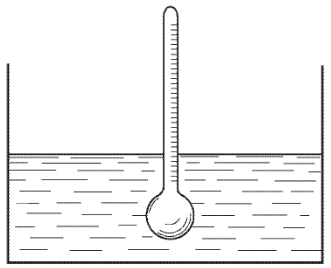
\includegraphics[width=0.35\textwidth]{areometr.png}
\caption{}
\label{areometr}
\end{figure}

\begin{ex} %Сив560
Ареометр с цилиндрической трубкой диаметра $D$ (рис. \ref{areometr}), плавающий в жидкости плотности $\rho$, получает небольшой вертикальный толчок. Найти период колебаний $T$ ареометра, если масса его $m$ известна. Движение жидкости и ее сопротивление движению ареометра не учитывать.
\begin{ans}
$T = 4 \sqrt{\pi m / g \rho D^2}$.
\end{ans}
\end{ex}	

\begin{figure}[h]
\centering
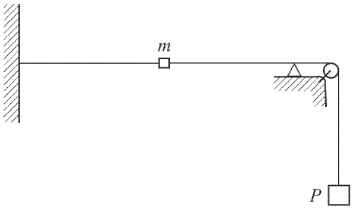
\includegraphics[width=0.5\textwidth]{oscilString.png}
\caption{}
\label{oscilString}
\end{figure}

\begin{ex} %Сив572
Найти период свободных малых колебаний грузика массы $m$, укрепленного на середине тонкой струны длины $L$ (рис. \ref{oscilString}). Массой струны можно пренебречь; натяжение струны постоянно и равно $P$.
\begin{ans}
$T = \pi \sqrt{m L /P}$.
\end{ans}
\end{ex}	

\begin{ex} %Сив580
Горизонтальная мембрана совершает синусоидальные колебания с круговой частотой $\omega$ и и амплитудой $A$. На мембране лежит маленький грузик. При каком условии грузик будет колебаться вместе с мембраной и при каком он начнет подскакивать?
\begin{ans}
При $\omega^2 A > g$ грузик будет подскакивать.
\end{ans}
\end{ex}	

\begin{figure}[h]
\centering
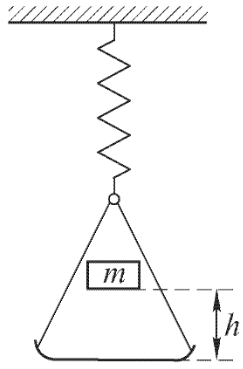
\includegraphics[width=0.25\textwidth]{fallingOnPlate.png}
\caption{}
\label{fallingOnPlate}
\end{figure}

\begin{ex} %Сив582
На чашку весов, подвешенную на пружине, падает с высоты $h$ груз массы $m$ и остается на чашке (рис. \ref{fallingOnPlate}), не подпрыгивая относительно нее. Чашка начинает колебаться. Коэффициент жесткости пружины $k$. Определить амплитуду $A$ колебаний (массой чашки и пружины по сравнению с массой груза можно пренебречь).
\begin{ans}
$A = \frac{mg}{k}\sqrt{ 1 + \frac{2hk}{mg}}$.
\end{ans}
\end{ex}	

\qualProblems

\begin{ex}
Предложите экспериментальный способ определения площади стола при помощи нитки, грузика и часов без использования линейки.
\end{ex}	

\begin{ex}
То, что пассажиры любого транспортного средства в момент торможения наклоняются вперёд по инерции, хорошо известно. Если быть внимательным, то можно заметить, что в момент торможения наклон пассажира вперёд сменяется наклоном назад. Таких толчков вперёд и назад может быть несколько. С чем это связано?
\end{ex}	

\begin{ex}
Какая часть периода требуется для того, чтобы тело, совершающее гармонические колебания, из положения равновесия первый раз пришло в крайнее положение?
\end{ex}	

\begin{ex}
Используя метод анализа размерностей физических величин определите зависимость частоты колебаний капли $\omega$ от ее плотности $\rho$, радиуса $r$ и коэффициента поверхностного натяжения $\sigma$.
\end{ex}	

\simpleProblems

\begin{ex}
Зависимость координаты колеблющейся точки от времени имеет вид $x = A\sin(\omega t/12)$. Известно, что в момент времени $t = 10$ с смещение равно 6 мм. Определите амплитуду колебаний (в мм).
\end{ex}	

\begin{ex}
Пружинный маятник совершает колебания, уравнение которых $x = 4\cos(\pi t + \pi/3)$ (см). Определите скорость и ускорение маятника через 20 с после начала движения. Масса маятника 200 г.
\end{ex}	

\begin{ex}
Математическому маятнику в положении равновесия сообщили некоторую скорость, и за 1/4 с она уменьшилась в 2 раза. Найдите длину маятника, считая возникшие колебания гармоническими.
\end{ex}	

\begin{ex}
Напишите уравнение гармонических колебаний груза массой $m = 100$ г, подвешенного на пружине жесткостью $k = 10$ Н/м, если амплитуда колебаний $A = 30 $ мм, а начальная фаза $\varphi_0 = \pi/4$.
\end{ex}	

\begin{ex}
Грузик массой $m = 200$ г, прикрепленный к горизонтальной пружине жесткостью $k = 20 $ Н/м, покоится на гладкой горизонтальной плоскости. Второй конец пружины закреплен. Грузику толчком сообщили горизонтальную скорость $v_0 = 1.0$ м/с, направленную вдоль оси пружины. Определите закон движения грузика $x(t)$, считая, что направление начальной скорости совпадает с положительным направлением оси $OX$.
\end{ex}	

\begin{ex}
Грузик массой $m = 200$ г подвешен на вертикальной пружине жесткости $k = 20$ Н/м. Его удерживают таким образом, что пружина остается недеформированной. В начальный момент времени груз освобождают, не сообщая ему начальной скорости. Определите закон движения грузика $x(t)$, считая, что ось $OX$ направлена вертикально вниз, а значение координаты $x = 0$ соответствует положению нижнего конца недеформированной пружины.
\end{ex}	

\begin{ex}
Гирька массой 0.3 кг, подвешенная на пружине жесткостью 15 Н/м, колеблется так, что ее максимальная скорость равна 2.8 см/с. Найдите амплитуду колебаний. Силами сопротивления пренебречь.
\end{ex}	

\begin{ex}
Максимальная скорость математического маятника при малых колебаниях $v_{\max} = 5 $ см/с, период колебаний $T = 1$ с. Определите максимальный угол отклонения маятника от вертикали в процессе колебаний.
\end{ex}	

\begin{ex}
Шарик массой 50 г, подвешенный на пружине, совершает гармонические колебания с амплитудой 10 см. Чему равна максимальная величина возвращающей силы (в мН), действующей на шарик, если циклическая частота колебаний 4 с\textsuperscript{-1}.
\end{ex}	

\begin{ex}
Точка совершает гармонические колебания вдоль прямой линии. При движении между крайними положениями средняя скорость оказалась равной $v = 4$ м/с. Найдите максимальную скорость.
\end{ex}	

\begin{ex}
Небольшое тело совершает гармонические колебания. Зная, что его максимальная скорость $v_{\max} = 9.42$ м/с, найдите величину средней скорости тела за время, в течение которого оно перемещается из одного крайнего положения в другое.
\end{ex}	

\begin{ex}
На горизонтальной пружине укреплено тело массы $M = 10$ кг, лежащее на абсолютно гладком столе. В это тело попадает и застревает в нем пуля массы $m = 10$ г, летящая со скоростью $v = 500$ м/с, направленной вдоль оси пружины. Амплитуда возникших при этом колебаний $A = 0.1$ м. Определите период возникших колебаний $Т$.
\end{ex}	

\begin{ex} %Сив577
На доске лежит груз весом $F = 10$ Н. Доска совершает гармоническое колебание в вертикальном направлении с периодом $T = 1/2$ с и амплитудой $A = 2$ см. Определить величину силы давления $F$ груза на доску. С какой амплитудой А должна колебаться доска, чтобы груз начал отскакивать от доски?
\begin{ans}
$A \approx 6,2$ см.
\end{ans}
\end{ex}	

\begin{ex} %Сив558
Найти выражения для потенциальной, кинетической и полной энергии материальной точки массы $m$, совершающей гармоническое колебание по закону $A \cos \omega t$.
\begin{ans}
$E_1 = m A^2 \omega^2 (1 - \cos 2 \omega t)/4$, $E_2 = m A^2 \omega^2 (1 + \cos 2 \omega t)/4$, $E = m A^2 \omega^2 /2$.
\end{ans}
\end{ex}	

\begin{ex} %Сив581
Доска совершает гармоническое колебание в горизонтальном направлении с периодом $P = 5$ с. Лежащее на ней тело начинает скользить, когда амплитуда колебания достигает величины $A = 0.6$ м. Каков коэффициент трения покоя к между грузом и доской?
\begin{ans}
$\mu = 4 \pi^2 A / (gT^2) = 0,1$.
\end{ans}
\end{ex}	

\complexProblems

\begin{ex} %Сив565
Представьте себе шахту, пронизывающую земной шар по одному из его диаметров. Найти закон движения тела, упавшего в эту шахту, учитывая изменения значения ускорения свободного падения внутри Земли. Трение о стенки шахты и сопротивление воздуха не учитывать.
\begin{ans}
Гармоническое колебание с периодом $T = 2 \pi \sqrt{R_0 / g_0}$, где $R_0$ -- радиус земного шара, $g_0$ -- ускорение свободного падения на поверхности Земли.
\end{ans}
\end{ex}	

\begin{figure}[h]
\centering
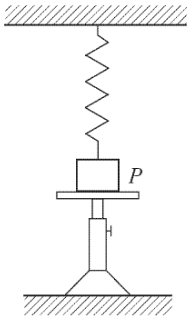
\includegraphics[width=0.25\textwidth]{removePlate.png}
\caption{}
\label{removePlate}
\end{figure}

\begin{ex} %Сив575
К пружине, один конец которой закреплен, подвешен груз $P$ массы $m$, лежащий на подставке так, что пружина не растянута (рис. \ref{removePlate}). Без толчка подставка убирается. Найти движение груза и максимальное натяжение пружины. Коэффициент жесткости пружины $k$.
\begin{ans}
$x = mg/k(1-\cos \sqrt{g/m} t)$.
\end{ans}
\end{ex}	

\clearpage